\section{Transformation to the $r$-$\varphi$ plane}
We have now seen that the ghosts are about $10^{-4}$ times less bright then their star, but potential exoplanets are even less bright. A Jupiter like exoplanet would be $10^{-9}$ less bright (reflecting light) and an Earth like even only $2 \cdot 10^{-10}$. Therefore the data must be really sensitive, with a high contrast and a high spatial resolution. As we can see in figure \ref{fig:ghosts} the star produces strong spiders and speckles which have similar brightness as the ghosts or are even brighter. Therefore exoplanets which are situated in this regimes cannot be detected, unless we are able to take out the signals of the spiders and speckles without taking away other signals, like the ones from exoplanets.\\
If we take a closer look at figure \ref{fig:ghosts} we observe that the structure of the spiders and the speckles are radially oriented around the star. In order to get rid of this effects it might be a good idea to transform the image into the r-phi plane, where we define the star to be at radius zero. After the transformation the spiders and speckles are distributed along the phi axis and they become weaker along the r axis. The image before and after the warping is shown in figure \ref{fig:warping_R150-300}, where we only warped the part of the image which is within radius 150 to 300 pixels. \\
\begin{figure}[H]
	\centering
		\subfigure[]{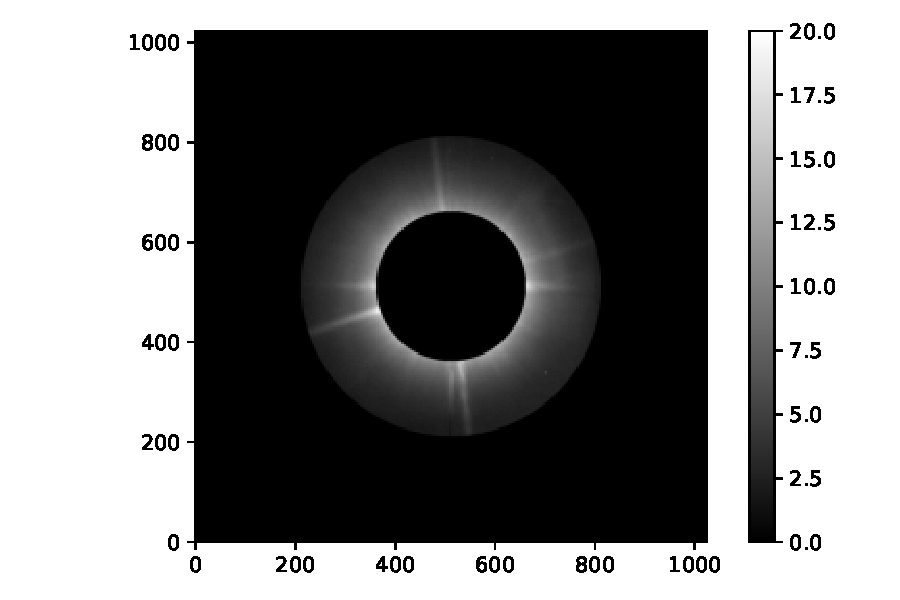
\includegraphics[width=0.6\textwidth]{pics/HDimg_R150_R300.pdf}}
		\subfigure[]{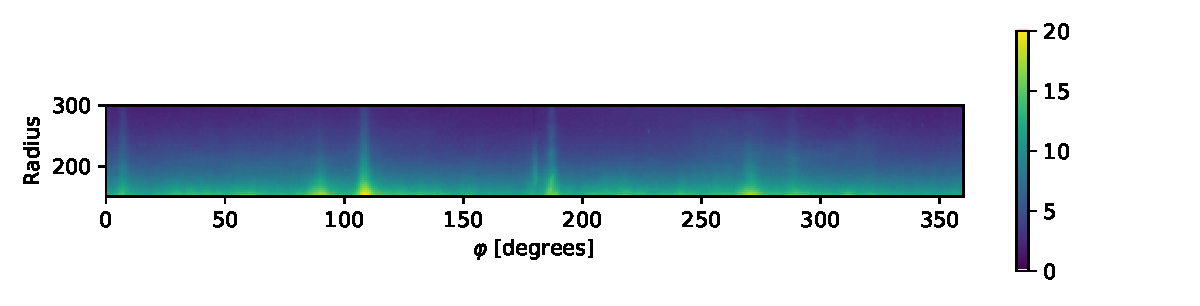
\includegraphics[width=1.1\textwidth]{pics/HDwarped_R150_R300.pdf}}
\caption{We mask the region (radius=150-300 pixels) which will be warped to the $r$-$\varphi$ plane (a). The resulting warped image (b), where we used spline interpolation.}
\label{fig:warping_R150-300}
\end{figure}
Lets have a look at how one can transform the image into the r-phi plane. This kind of transformation is called image warping in image processing. In our case the image warping is based on a specific transformation, namely the transformation from Cartesian to polar coordinates and is therefore also called polar-cartesian distortion.\\
In general an image warping is based on a transformation $T: \mathbb{R}^2 \rightarrow \mathbb{R}^2$, such that 
\begin{equation}
	\vec{x} \mapsto \vec{u} = \begin{pmatrix} T_u(x,y) \\ T_v(x,y) \end{pmatrix},
\end{equation}
where $\vec{x} = \begin{pmatrix} x \\ y \end{pmatrix}$ and $\vec{u} = \begin{pmatrix} u \\ v \end{pmatrix}$. When we want to warp an image $f$ into an image $g$ we do the following calculation
\begin{equation}
	g(\vec{u}) = g(T(\vec{x})) = f(\vec{x}).
\end{equation}
This means that at pixel $\vec{u}$ the computed image $g$ has the same intensity as the original image $f$ at pixel $\vec{x}$. \cite{ImageWarping}\\
When we want to describe the position of a pixel we use Cartesian coordinates, the way it is shown in figure \ref{fig:CoorinateSystems} (a), but there are also other ways to describe the location of the pixels. Figure \ref{fig:CoorinateSystems} (b) shows the image with a polar coordinate system, where we chose the origin to be in the center (where the stars position is).
\begin{figure}[H]
	\centering
		\subfigure[]{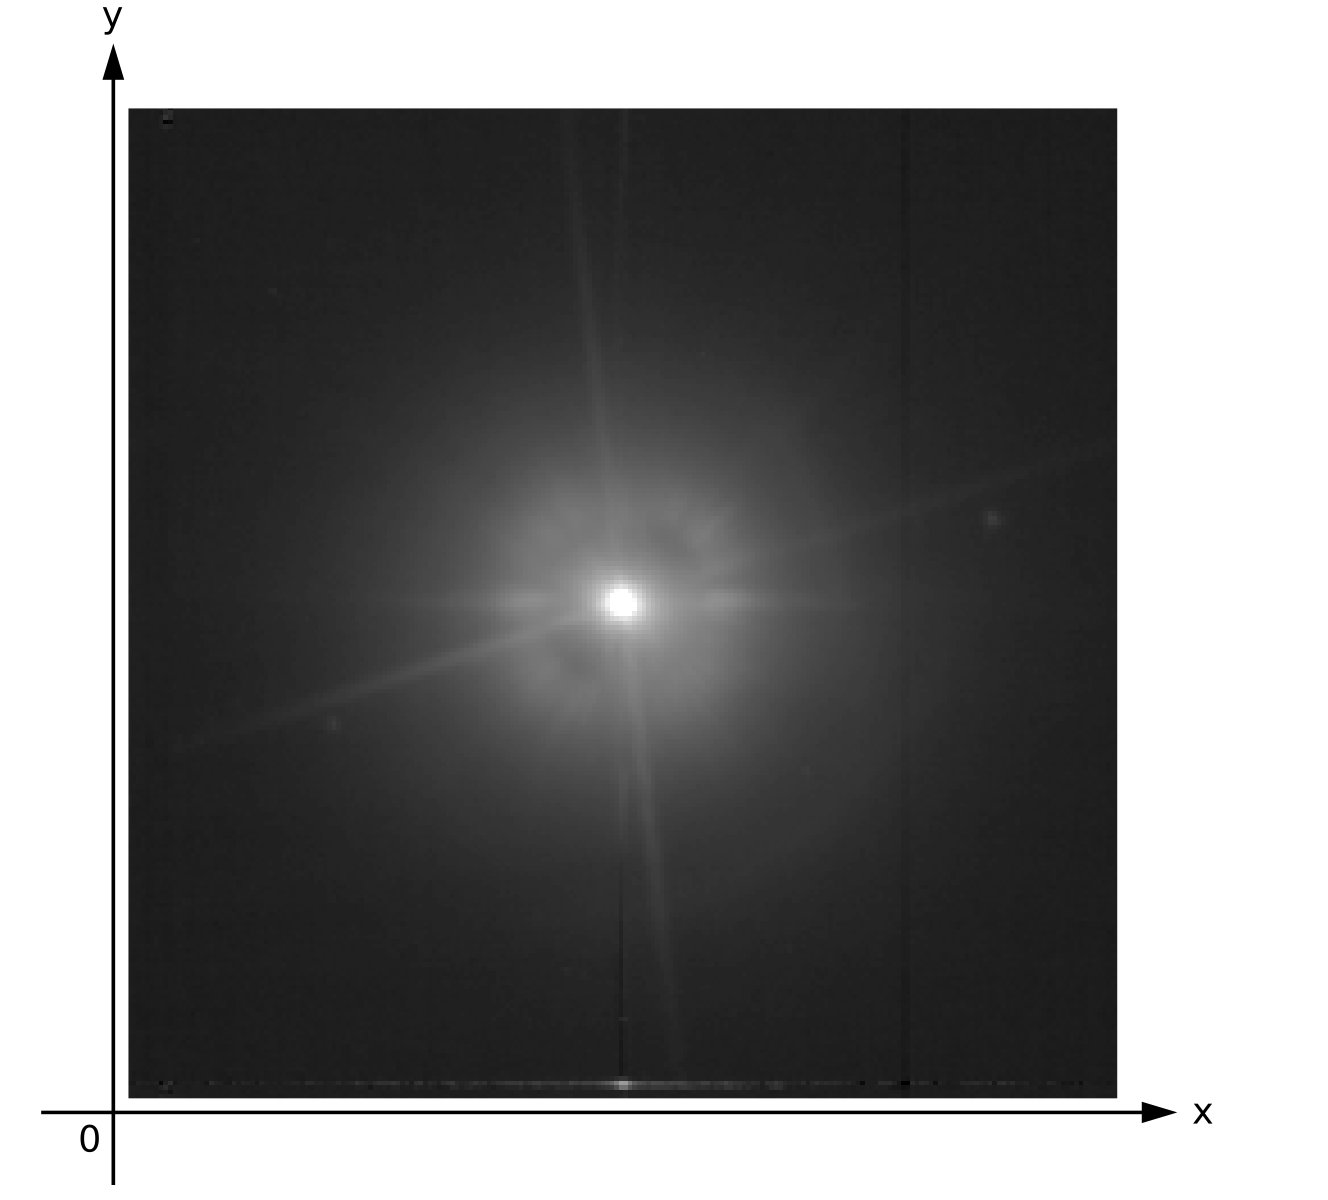
\includegraphics[width=0.49\textwidth]{pics/Star_CartesianCoor.png}}
		\subfigure[]{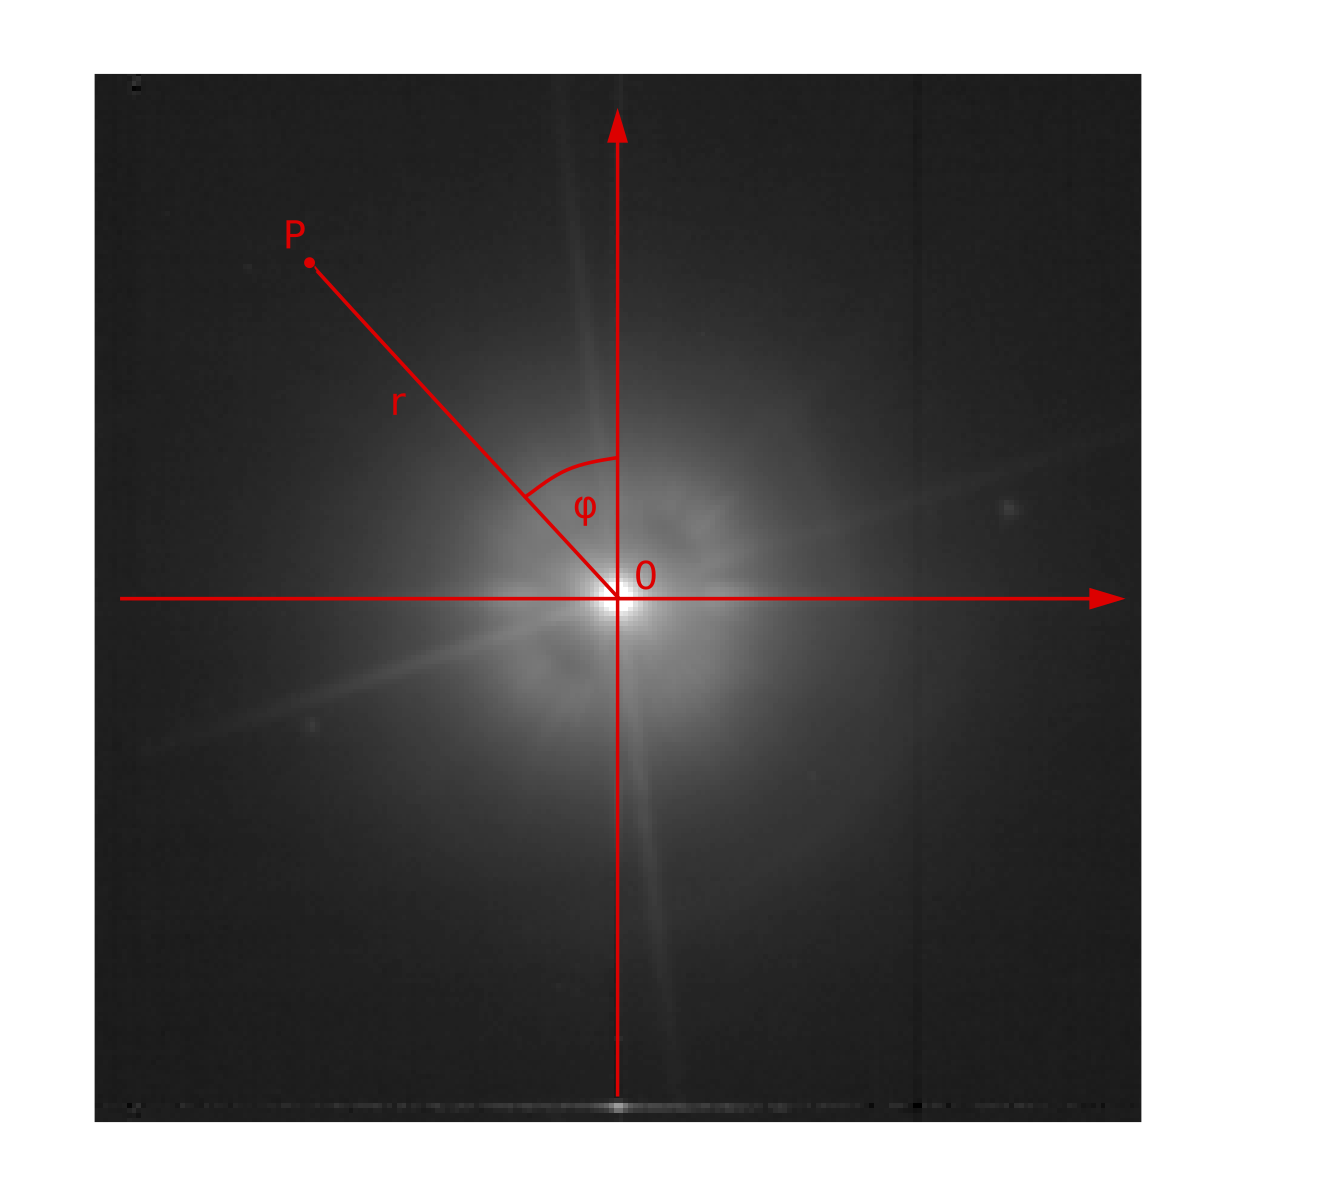
\includegraphics[width=0.49\textwidth]{pics/Star_PolarCoor.png}}
\caption{To describe the location of pixels in an image one usually uses Cartesian coordinates (a), but we can also use polar coordinates (b).}
\label{fig:CoorinateSystems}
\end{figure}
In order to change from Cartesian coordinates $x, y \in \mathbb{R}$ to polar coordinates $r \in [0, \infty)$, $\varphi \in [0, 2\pi)$ one needs to do the following calculations:
\begin{equation}
	r = \sqrt{x^2 + y^2}\\
	\varphi = \arctan \left( \frac{-x}{y} \right).
\end{equation}
For the back transformation from polar to Cartesian coordinates we compute
\begin{equation}
	x = -r \sin(\varphi)\\
	y = r \cos(\varphi).
\end{equation}
The transformation of the pixels from Cartesian to polar coordinates results in pixels which are not squares. However for our resulting image in the $r$-$\varphi$ plane, we need square pixels. This pixel distortion happens because the number of pixels included at a certain radius away from the center increases proportionally to the radius. This means that there are twice as many pixels at a radius of $100$ (pixels) than at radius $50$. We now have two options after we have defined the grid of our $r$-$\varphi$ plane. Either we choose the grid such that at $r=r_{max}$ every pixel in the grid corresponds to a pixel in the original image and for smaller radii we have pixel which are empty. Or we choose the size of the grid differently and use interpolation to assign an appropriate value to each pixel in the $r$-$\varphi$ plane. We decided to use interpolation, since we cannot work with the data if there are empty pixels. In figure \ref{fig:warping_R150-300} we have already seen an example for this transformation using spline interpolation.\\
Now lets think about which length the grid should have. Since our main interest is to find round objects like exoplanets, it would be beneficial if round objects are still round after the transformation. In order for this to be satisfied, the number of pixels at the radius position of the object has to stay unchanged. We therefore decided to choose the radius range (the $\varphi$ angle goes from $0$ to $360$ degrees and thus covers the whole circle), such that the object we want to examine is in the middle and the grid size corresponds to the length of the radius range, i.e. for $r_{min}=100$ and $r_{max}=300$ the length of the grid the radius direction is $r_{len}=r_{min}-r_{max}=200$. The resulting grid size in $\varphi$ direction depends then on the chosen radius range. Namely such that: $\varphi_{len} = 2\pi \cdot (r_{min}+\frac{r_{len}}{2})$.\\
Figure \ref{fig:Circle_distortion} illustrates the effect of this transformation onto circles in the original image (a). In the center of the warped image at $r=200$ the number of pixels is unchanged by the transformation, this means no interpolation nor averaging was needed. Therefore circles stay circles, if they are placed in the middle of the warped image, see figure \ref{fig:Circle_distortion} (c). If we go to larger radii the number of pixels per radius (in original image) increases. Since in the warped image all radii have the same number of pixels $r_{len}$ the transformation averages the information in the original pixels into fewer pixels and the circle becomes elliptic like in its shown in figure \ref{fig:Circle_distortion} (b). The opposite effect happens if we go to smaller radii where the number of pixels per radii (in original image) decreases and interpolation is needed to distribute the original information to an enlarged number of pixels. This results also in an elliptic shape, but with the semi-major axis now in the $\varphi$ direction, see figure \ref{fig:Circle_distortion} (d). 
\begin{figure}[H]
	\centering
		\subfigure[]{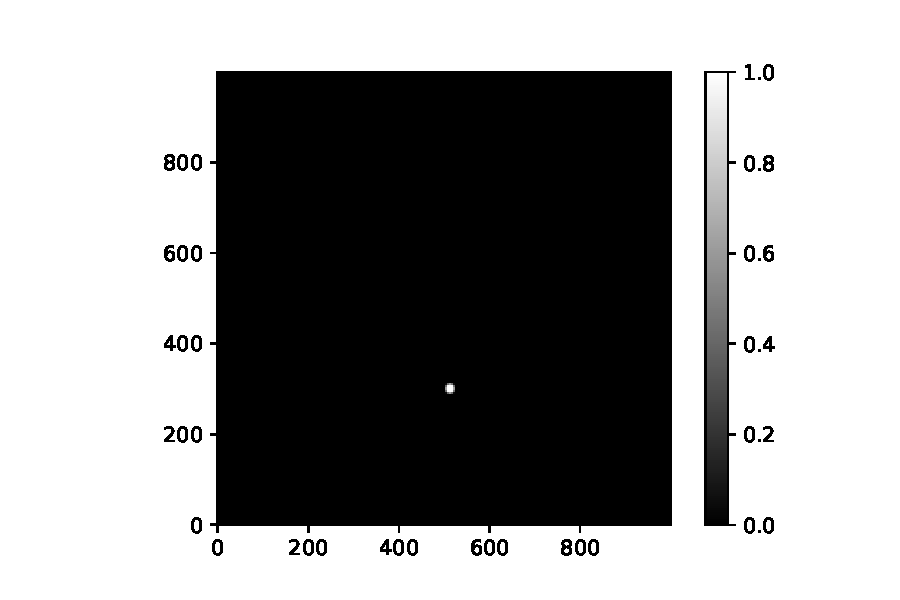
\includegraphics[width=0.6\textwidth]{pics/Circle_image.pdf}}
		\subfigure[]{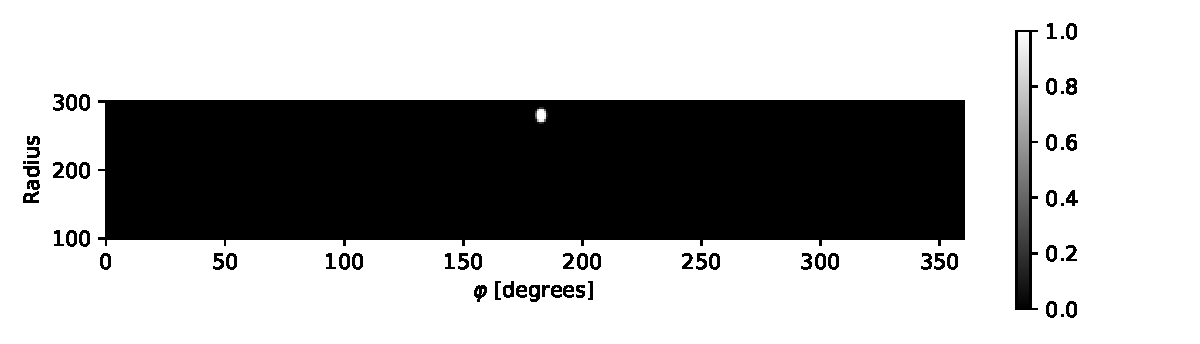
\includegraphics[width=1.1\textwidth]{pics/Circle_top.pdf}}
		\subfigure[]{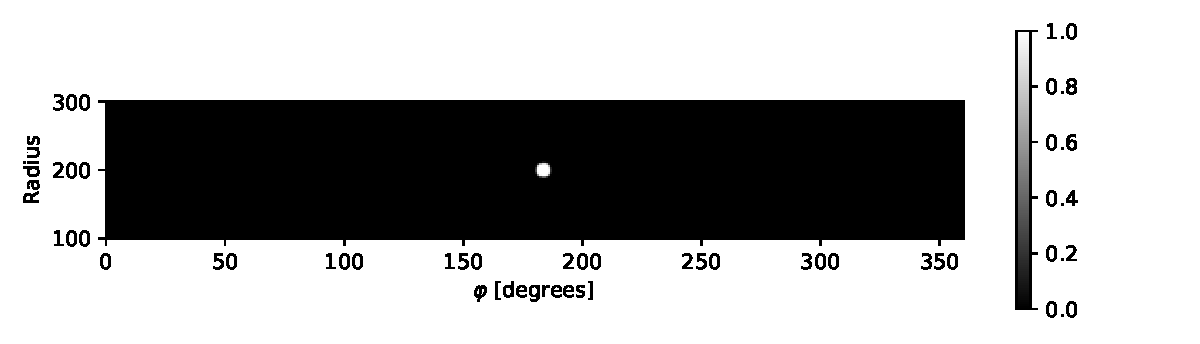
\includegraphics[width=1.1\textwidth]{pics/Circle_center.pdf}}
		\subfigure[]{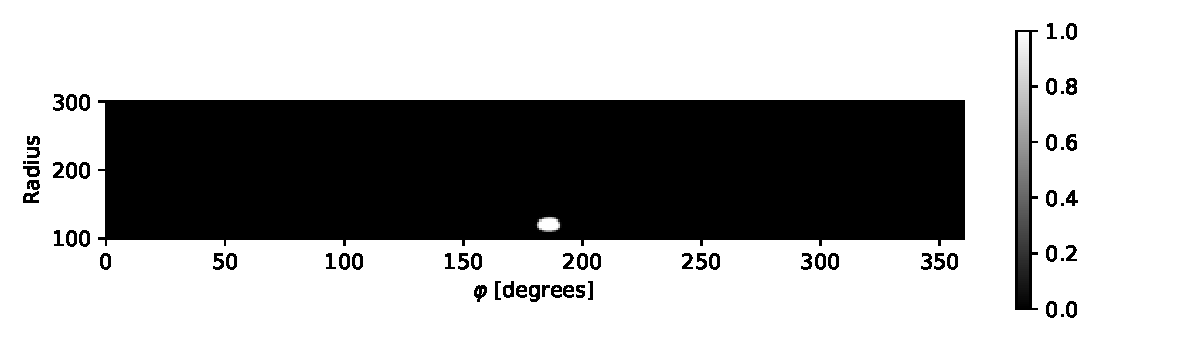
\includegraphics[width=1.1\textwidth]{pics/Circle_bottom.pdf}}
\caption{The warping is defined such that a point in the original image (a) is left unchanged, if it is in the middle of the radius range of the transformed image (c). Otherwise the point will become an ellipse (b) and (d).}
\label{fig:Circle_distortion}
\end{figure}
In order to perform the transformation to the $r$-$\varphi$ plane, we need to define the new shape of the warped image, as discussed before. From this we then define the new pixel grid in polar coordinates and then assign the corresponding Cartesian coordinate values. With this information it is already possible to map the values of the pixels in the original image to the warped one. In our program (shown below \cite{ImageWarping}) we used the python package scipy.ndimage.map\_coordinates() which uses cubic spline interpolation to do the mapping.\\
As we already mentioned interpolation is used to assign a value to every pixel in the new frame by using the information from the old frame. Or in other words the wholes (where we have no information) are closed by cleverly inventing new values for these wholes through the observation of the information in the neighborhood of the whole. The used spline interpolation fits polynomials to the known values (in our case third order polynomials) in the neighborhood and takes then the values given by the polynomials. We chose this method, because we received the best results with it, but one can also use different interpolation methods like nearest neighbor interpolation or the bilinear interpolation. 
\lstset{language=Python, numbers = none}
\begin{lstlisting}[frame=lines]
def to_rphi_plane(image, im_shape, r_min, r_max):
    """
    Warping to r-phi plane.

    Parameters
    ----------
    image : float32, np.array 
        An intensity image.
    im_shape : (int, int)
        Shape of image f.
    r_min : int
        Inner radius.
    r_max : int
        Outer radius.

    Returns
    -------
    warped : float32, np.array 
        r-phi plane image. 

    """
    # Define the shape of the resulting warped image
    r_len = r_max - r_min
    phi_len = int(2*np.pi*(r_min + r_len/2))
    
	# Define the new grid    
    rs, phis = np.meshgrid(np.linspace(r_min, r_max, r_len), 
                           np.linspace(0, 2*np.pi, phi_len), sparse=True)
    
    # Assign the corresponding Cartesian coordinates to the new grid
    xs, ys = rphi_to_xy(rs, phis)
    xs, ys = xs + im_shape[0]/2 -  1, ys + im_shape[1]/2 - 1
    xs, ys = xs.reshape(-1), ys.reshape(-1)
    coords = np.vstack((ys, xs))
    
    # Create the warped image with spline interpolation 3th order
    warped = scipy.ndimage.map_coordinates(image, coords, order=3)
    warped = g.reshape(phi_len, r_len)
    
    return warped
\end{lstlisting}
It is also possible to transform the image back to the Cartesian coordinate map. By simply doing a warping of the image in the $r$-$\varphi$ plane back to the original $x$-$y$ plane.\\
Lets go back to our example with the circle and have a look if the aperture flux of the circle is preserved trough the warping of the image. We find that the circle has an aperture flux of $306$, after the transformation to the $r$-$\varphi$ plane this aperture flux is $302$. So the aperture flux does not change much through the transformation. After the back transformation we get an aperture flux of $306$ which is the same as in the original image. Still we also need to check for this in our data, where we have smooth transitions. We do so by using ghost 1 which is at a radius of $390$ pixels in the data of HD142527. For the flux of the aperture in the image we get $231.5$. After a transformation to the $r$-$\varphi$ plane where we chose $r_{min}=290$ and $r_{max}=490$ the flux of the aperture was $232.1$. So we can say that the transformation conserves the aperture flux which is a really good and important property.
